\begin{figure*} 
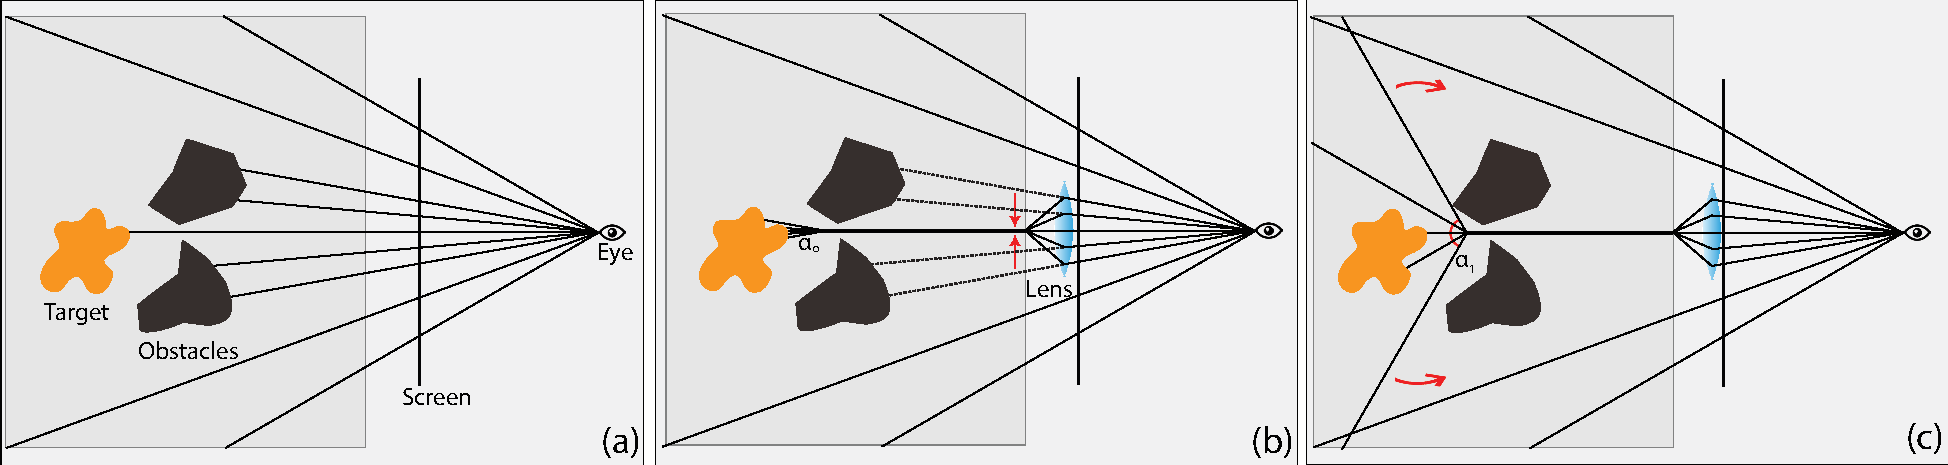
\includegraphics [width=\textwidth]{images/principle.pdf} 
\caption{The mechanism of the obstruction-free fish-eye lens. (a) The classic ray-casting where an interesting feature is partially hidden by other items in front of it. (b) The first main step: The lens makes converge the rays to avoid the obstacles. Once they are close to the target, the rays follow again their initial trajectory (with the initial angle) of view $\alpha_0$. Only a small part of the target is visible and magnified. (c) The target become visible by increasing the angle of view to $\alpha_1 \in \left[120,180\right]$.   }
\label{f:fisheye}
\end{figure*}


Thanks to various rendering techniques, volumetric data can be displayed in many different fields (engineering, material sciences, medical imaging, etc.). Direct volume rendering techniques or isosurfaces techniques render these volumes into graphical representations in order to allow their exploration. In volume rendering, occlusion management is a challenge. As such, in 3d representations of volumes, some areas or objects (subsets) can be partially or fully hidden by others because of their locations.

Global techniques such as transfer functions,  segmentation, and selection/clipping are used to remove occlusion in the entire volume. Therefore, they are a good way to reduce occlusion and make visible interesting features.  However, it is still difficult to create a good transfer function/segmentation  especially when the data are heterogeneous. In fact, designing a good transfer function depends heavily on the type of dataset and on the user's purpose. For instance, in the field of baggage inspection, the variation of densities prevents to create a unique transfer function for each baggage. In contrast, it is easier to design a good transfer function for a system dedicated to visualizing the same type of datasets (brain CT scans, bone tissues, etc.). 

Many studies propose different tools and interaction techniques to by-pass occlusion issues in 3D environments such as lenses, deformations ~\cite{595268}, augmented reality, etc. Lenses, which are flexible lightweight tools that enable local and temporary modifications of the visualization, are suitable to deal with occlusion while keeping information about the global context. This is a good local solution for occlusion problems and an interesting way to keep the user aware of the global meaning of the dataset. Thus, while most lenses in volume rendering are used to magnify a volume subset~\cite{CGF:CGF12871}, we propose a focus+context (F+C) lens that combines a distortion technique which pushes aside the occluding objects, and a  fish-eye field of view in order to provide a better perspective on partially occluded items of interest in the volumes.  


Furthermore, performances are still a  challenge in volume rendering systems. In fact, depending on the size of the dataset and also the resolution of the resulting produced image: the rendering process can be very slow. Some optimization strategies such as empty space skipping~\cite{Liu:2009:AVR:2421899.2421919}, early ray termination~\cite{CGF:CGF12605}, multiple and adaptive resolutions allow to speed up the rendering process by increasing the frame rate. With the advent of CUDA as a higher-level GPU programming language, CUDA-based ray-casters were introduced~\cite{Kainz:2009:RCM:1661412.1618498}. So, in order to support our focus+context interactive lens, our volume visualization system relies on a CUDA-based ray-casting algorithm~\cite{Roettger:2003:SHV:769922.769948}.  This framework enables volumetric datasets visualization and offers a set of interactive tools including our lens for the purpose of easing the exploration and the manipulation of the data.

The structure of this paper is as follows. Section 2 presents related work in the areas of ray-casting, occlusion management, lenses and deformations. Section 3 describes the principle of our lens. Section 4 presents a method to convert vector datasets into a volume. Section 5 illustrates our lens technique with 3 scenarios. Section 6 discusses the presented technique. Finally, section 7 concludes the paper. 